\documentclass{cilamce19}

\begin{document}
%Insert the header


%%This is the short title that will be inside the header 
\shorttitle{Put your short title in here.}
 
\begin{titlepage}
	
	\newgeometry{top=1.3in,bottom=0.8in,right=0in,left=2in}

	
	\begin{figure}
	\flushright
	
\includegraphics[width=2.25in]{clm19_lb.png}
    \end{figure}


 \begin{center}
 	\begin{title}
 		\centering
 		\textbf{INSTRUCTIONS FOR PREPARATION AND SUBMISSION OF FULL-PAPERS FOR PUBLICATION IN THE PROCEEDINGS OF XL CILAMCE AND STARTS CILAMCE19.CLS V1.01}
 	\end{title}	
 \end{center}



%Authors and Affiliations
\textbf{First A. Author}
\\
\textbf{Second B. Author}
\\
\textit{somebody1@somewhere.com}\\
\textit{somebody2@somewhere.com}
\\
\textbf{Affiliation}
\\
\textit{Address, Zip-Code, State/Province, Country}
\\
\textbf{Third C. Author}
\\
\textit{somebody3@elsewhere.com}\\
\textbf{Affiliation}
\\
\textit{Address, Zip-Code, State/Province, Country}
\\

%Abstract
\noindent %Abstract should not be indented
\textbf{Abstract:} This document-template provides detailed instructions for preparing and submitting a paper to the XL Ibero-Latin American Congress on Computational Methods in Engineering (CILAMCE-2019). Please follow these general instructions carefully: (a) type the body of the paper in single column; (b) use no more than 20 A4-size pages (maximum 5 pages for papers at the Research Beginners Mini-symposium), each formatted with 2.5 cm margins on all sides (do not insert page numbers); (c) use 11pt Times New Roman throughout the body of the text, with 13 pt for the title andfirst-level headings (we strongly encourage you to use the pre-defined styles of this template, as they embed all necessary text formatting for the corresponding paragraph type); (d) type up to 250 words in the abstract; (e) always use either single-spaced orexactly 13-pt-spaced lines, with justified alignment; (f) cite references by Name [number],and list them consecutively in the reference list by the order of citationin the text (the list should only include works that are cited in the text); (g) provide good quality figures; (h) define all quantities, variables and symbols as soon as they first appear in the text; (i) equations must be typed either in Math type or MS Equation (or similar); (j) use only SI units. It is strongly recommended that the paper be written in English. Papers in Portuguese, Spanish or Italian may be occasionally accepted, provided that at least the abstract and the slides for oral presentation are in English

\noindent %keywords should not be indented
%Keywords
\textbf{Keywords:} First keyword, Second keyword, Third keyword (up to 5 keywords) 

\end{titlepage}




%Here your work really starts.
\section{Introduction}
   All full-length papers that have been orally presented at the XL CILAMCE will be published in the congress proceedings.It is extremely important that you prepare the digital version of your contribution in strict accordance with the present instructions.After the preparation of your paper you should generate a PDF file for submission. Only PDF files will be accepted by the online submission system.
   



\section{Typing instructions}

The paper must be written preferably in English. Papers in Portuguese, Spanish or Italian may be occasionally accepted, provided that at least the abstract and the slides for oral presentation are in English. The number of non-English contributions should be kept to a minimum, as we encourage the authors to adopt English as the main conference language as much as possible.

 
 


\subsection{Paper length} 
The full-paper including figures and tables should not exceed 20 A4-size pages (maximum 5 pages for papers at the Research Beginners Mini-symposium). Please limit your paper by writing concisely, rather than by reducing figures or tables to a size at which symbols/labels would become difficult to read. The final PDF file should not exceed 3 MB.



\subsection{Page format}
Each A4-size page should be formatted with 2.5 cm margins on all sides. This defines the printable area. Inside this area, the text must be arranged in a single column. Please do not print any border around the text and do not insert page numbers.The general appearance of the paper should look like this document.


\subsection{Genreal text specifications}
The body of the text must be typed using 11pt Times New Roman throughout, as in the present document. This includes also second-level headings (as in Section 2.3 above), figure and table captions. The first page must include the paper title, authors, affiliations, abstract and keywords. The body of the text must begin in the second page.We encourage you to use the pre-defined styles of this template, as they embed all necessary text formatting for the corresponding paragraph type.


\textbf{Remark 1: Paper title.} The title should be in boldface type, 13 pt capital letters (all) and justified on the page, and must not exceed three lines. It should be single spaced. Please pay attention to the 18 pt line spacingafter the title and before the first author.

\textbf{Remark 2: Author(s) and affiliation(s).} Type authors names in boldface type, flush left, one per line, including first name, middle initial(s) and last name. Each name or group of names must be followed by the corresponding emails and affiliations, which should be both in italics.

\textbf{Remark 3: Abstract and keywords.} Type Abstract in boldface, flush left, followed by a period. On the same line, type the abstract in regular (plain) format, justified alignment. The abstract should be no longer than 250 words. Please pay attention to the 18 pt line spacing between the authors affiliations and the abstract, as well as between the abstract and the keywords. For the keywords, type the heading Keywords, followed by a colon, in boldface, flush left and type 3 to 5 keywords, separated by commas, with only the first letter of each keyword capitalized.

\textbf{Remark 4: Headings.} First-level headingsmust be typed in sentence letters, 13 pt boldface type, flush left, as in Section 2 above. Use Arabic numbering (if you use this template's styles, the automatic numbering is already assigned to the first-level heading style). Notice the 18 pt line spacing before and after first-level headings. For second-level headings, use sentence letters, 11 pt boldface type, flush left, with Arabic double numbering (if you use this template's styles, the automatic double numbering is already assigned to the second-level heading style). Notice the 13 pt line spacing before and after second-level headings. Do not use third-level headings. Instead, at most, Remarks (or the like) are allowed, as shown here. These shall start with the word Remark (or the like)in boldface italics, followed by a number and title. The text that follows must be in regular (plain) format. Notice the 13 pt line spacing before and after remarks.

\textbf{Remark 5: Body of text.} As said before, the body of the text should be typed in 11pt Times New Roman, using either single-spaced or exactly 13-pt-spaced lines, and justified alignment. Start each paragraph with an indentation of 0.75 cm from the left margin, and allow no space between paragraphs. 


\subsection{Equations, symbols and units} 
Equations must be typed in Math type or MS Equation (or any equivalent equation editor). They must be centered, right-numbered, with numbers enclosed in parentheses and placed flush right. Allow 6 pt line spacing before and after an equation. For example:

\begin{eqnarray}
q =-4 \theta^{2} \frac{T}{c}
\label{eq1}
\end{eqnarray}

Please pay attention to the punctuation after the equations, as equations are part of the text and must be punctuated accordingly.

When referring to an equation in the text, write Eq. (\ref{eq1}) (without the quotation marks), except at the beginning of a sentence, where in  Equation (1) should be used (again, without quotation marks). Please describe the notation adopted and be careful as to define all quantities, variables and symbols as soon as they first appear in the text. A nomenclature section is not necessary.

All data, including those shown in tables and figures, must be reported in SI units. Decimal points rather than commas should always indicate decimals.


\subsection{Figures and tables}

Figures and tables should be inserted as close as possible to their mentioning in the text. Enclosed text and symbols must be clearly readable; avoid small symbols thus. Supply good quality pictures and illustrations.Figures and tables and their captions should be centered in the text. Place figure captions below the figures and allow 6 pt line spacing between both, and 13 pt line spacing after the caption (before the adjacent text). Place table title above the table, leaving 13 pt line spacing before the title and 6 pt between the title and the table.

\begin{table}[H]
		\caption{Table made in \tex. To compile this you must have tex-science package on your system.}
\begin{tabular}{SSSSSSSS} \toprule
	{$m$} & {$\Re\{\underline{\mathfrak{X}}(m)\}$} & {$-\Im\{\underline{\mathfrak{X}}(m)\}$} & {$\mathfrak{X}(m)$} & {$\frac{\mathfrak{X}(m)}{23}$} & {$A_m$} & {$\varphi(m)\ /\ ^{\circ}$} & {$\varphi_m\ /\ ^{\circ}$} \\ \midrule
	1  & 16.128 & +8.872 & 16.128 & 1.402 & 1.373 & -146.6 & -137.6 \\
	2  & 3.442  & -2.509 & 3.442  & 0.299 & 0.343 & 133.2  & 152.4  \\
	3  & 1.826  & -0.363 & 1.826  & 0.159 & 0.119 & 168.5  & -161.1 \\
	4  & 0.993  & -0.429 & 0.993  & 0.086 & 0.08  & 25.6   & 90     \\ \midrule
	5  & 1.29   & +0.099 & 1.29   & 0.112 & 0.097 & -175.6 & -114.7 \\
	6  & 0.483  & -0.183 & 0.483  & 0.042 & 0.063 & 22.3   & 122.5  \\
	7  & 0.766  & -0.475 & 0.766  & 0.067 & 0.039 & 141.6  & -122   \\
	8  & 0.624  & +0.365 & 0.624  & 0.054 & 0.04  & -35.7  & 90     \\ \midrule
	9  & 0.641  & -0.466 & 0.641  & 0.056 & 0.045 & 133.3  & -106.3 \\
	10 & 0.45   & +0.421 & 0.45   & 0.039 & 0.034 & -69.4  & 110.9  \\
	11 & 0.598  & -0.597 & 0.598  & 0.052 & 0.025 & 92.3   & -109.3 \\ \bottomrule
\end{tabular}
\label{tab1}
\end{table}


Arabic numerals should be used in figures and tables (e.g., Figure 1, Figure 2, Table 1, Table 2, etc). Refer to them in the text as Table \ref{tab1} and Fig. 1 (no quotation marks), except at the beginning of a sentence, where in Figure 1 should be used (again, no quotation marks).


\begin{figure}[H]
	\centering
	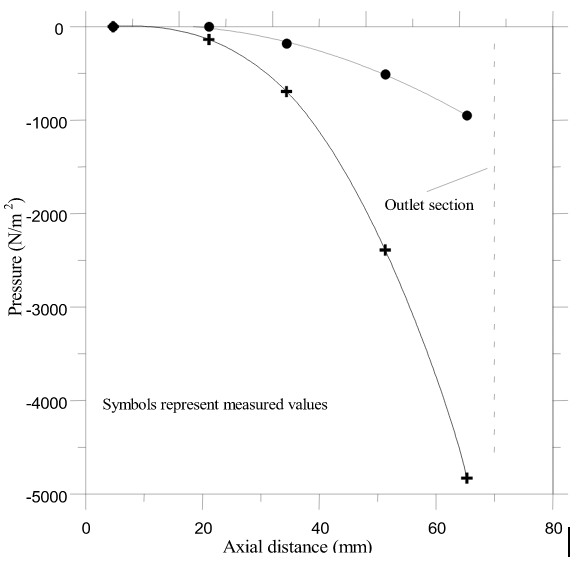
\includegraphics[scale=2]{Images/fig1.png}
	\caption{Pressure variation along the nozzle: experimental data}
	\label{fig1}
\end{figure}


When constructing graphs or plots, do not forget to label coordinates and statethe corresponding units. Similarly, label all columns/rows in tables and state corresponding units whenever applicable.

\subsection{Permission}
You are responsible for making sure that you have the right to publish everything in your paper. If you use material from a copyrighted source, you may need to obtain permission from the copyright holder.

\subsection{References}

References should be cited in the text by Name [number]. For example: In a recent work, \citet{book-example}, \citet{inbook-example} and \citet{article-example}  proposed \dots. Numbers must be Arabic, enclosed in square brackets and used consecutively. References must be listed at the end of the paper, in a separate section entitled References. They must be listed consecutivelyby the order of citation in the text. Type the word References in boldface, 13 pt Times New Roman type from the left margin, leaving 18 pt line spacing before and after. Type the reference list below it, in 11 pt Times New Roman (please do not leave blank spaces between references).See examples below. The list should only include works that are cited in the text. 

\section*{Acknowledgements}
This section should be positioned right before the reference list. Type Acknowledgements in boldface, 13 pt Times New Roman type from left margin, leaving 18 pt line spacing before and after.



  \bibliography{references.bib}
  
\end{document} 
